\documentclass[8pt]{article}
\usepackage[letterpaper,margin=0.18in]{geometry}
\usepackage[T1]{fontenc}
\usepackage{lmodern}
\usepackage{microtype}
\usepackage{amsmath,amssymb,mathtools}
\usepackage{booktabs,array,multicol}
\usepackage{xcolor}
\usepackage{enumitem}
\usepackage{fancyhdr}
\usepackage{graphicx}

\definecolor{ink}{HTML}{183B4D}
\definecolor{accent}{HTML}{176B87}
\pagestyle{fancy}
\fancyhf{}
\lhead{\textcolor{ink}{\textbf{Data Mining | Test 1 Notes}}}
\rhead{\textcolor{ink}{\thepage}}
\renewcommand{\headrulewidth}{0pt}
\setlength{\headheight}{9pt}
\setlength{\parindent}{0pt}
\setlength{\parskip}{1pt}
\setlength{\columnsep}{0.13in}
\setlist{nosep,leftmargin=1.05em}
\setlist[itemize]{itemsep=0pt}
\setlist[enumerate]{itemsep=0pt,leftmargin=1.2em}
\renewcommand{\arraystretch}{0.9}
\setlength{\abovedisplayskip}{2pt}
\setlength{\belowdisplayskip}{2pt}
\setlength{\abovedisplayshortskip}{1pt}
\setlength{\belowdisplayshortskip}{1pt}

\newcommand{\sect}[1]{\vspace{1pt}\textcolor{accent}{\textbf{\normalsize #1}}\par\vspace{1pt}\hrule height 0.35pt\vspace{0pt}}
\newcommand{\term}[1]{\textbf{#1}}
\newcommand{\code}[1]{\texttt{#1}}

\begin{document}
\scriptsize
\begin{multicols*}{2}

\sect{Data + Questions}
\term{Observational unit}: one row/record. \term{Population}: broader units/process of interest; observed data are not automatically the population. \term{Group}: category used to compare. \term{Outcome}: measured response. \term{Context}: structure to preserve (e.g., region/weekend). \term{Point estimate}: one statistic from observed data.

\term{Workflow:} question + unit $\rightarrow$ group/outcome/context $\rightarrow$ inspect shape, types, missingness, labels $\rightarrow$ choose statistic before testing $\rightarrow$ summarize/visualize $\rightarrow$ state sampling/dependence limits $\rightarrow$ simulate reproducibly $\rightarrow$ interpret in original units.

\term{Description $\ne$ causation}: an observed group difference does not prove group membership caused it. Generalization needs representative sampling; causation needs appropriate design/assumptions.

\begin{tabular}{@{}p{0.25\linewidth}p{0.69\linewidth}@{}}
\toprule
Statistic & Meaning \\
\midrule
Mean diff. & $\bar x_A-\bar x_B$: average magnitude; sensitive to extremes.\\
Median diff. & $\widetilde{x}_A-\widetilde{x}_B$: middle; less outlier-sensitive.\\
Rate diff. & $\hat p_A-\hat p_B$: fraction above threshold/Boolean condition.\\
Quartile diff. & $Q_{.75,A}-Q_{.75,B}$: upper distribution, not maximum.\\
\bottomrule
\end{tabular}

Always state subtraction order, units, and missing-value handling. Mean of a Boolean condition $=$ proportion true: \code{(x > c).mean()}.

\sect{Permutation Tests}
\term{Purpose}: test evidence against a no-association null model. Under $H_0$, outcomes and labels are unrelated; reassignment creates null worlds.
\begin{enumerate}
\item Choose question-matched statistic $T$.
\item Calculate observed $T_{obs}$.
\item Identify what must remain fixed (group sizes; strata if relevant).
\item Reassign labels under $H_0$; recompute $T$.
\item Null distribution $=$ simulated statistics; compare to $T_{obs}$.
\end{enumerate}
\term{Exchangeability}: units may be shuffled only when the null makes them interchangeable. Stratify/permutate within region or other design cells when that structure must remain fixed. Ask: what relationship is broken, and what is preserved?
\[
\hat p=\frac{\#\{T^*\text{ at least as extreme as }T_{obs}\}+1}{B+1}
\]
Two-sided: extreme in either direction, usually $|T^*|\ge|T_{obs}|$. Resolution floor $\approx1/(B+1)$. A p-value is not $P(H_0\mid\text{data})$ and not the probability the result happened ``by chance.''

\term{Interpretation:} Under the null model represented by the procedure, about $p$ of reassignments produced a statistic at least as extreme as observed; this is [weak/strong] evidence against no association for these units, subject to exchangeability and sampling assumptions.

\sect{Bootstrap}
\term{Purpose}: estimate sampling variability by treating observed data as an empirical population. Resample observed units \term{with replacement}, usually separately within groups; preserve each group sample size.

\term{Point estimate}: original statistic. \term{Bootstrap sample}: one resampled dataset. \term{Replicate}: statistic from one bootstrap sample. \term{Distribution}: all replicates. \term{SE}: SD of replicates. \term{95\% percentile CI}: $[q_{.025},q_{.975}]$.

\term{Bootstrap Interval}: If the recorded groups reasonably represent their target populations and the resampling assumptions are
reasonable, the interval gives plausible values for the population difference under the method’s long-run
coverage interpretation. It is not the probability that a fixed parameter is random, and it does not repair
biased or unrepresentative data.

\begin{tabular}{@{}p{0.29\linewidth}p{0.65\linewidth}@{}}
\toprule
Permutation & Bootstrap \\
\midrule
Test no association & Estimate variability/uncertainty \\
Null world; labels reassigned & Empirical world; values resampled \\
Typically no value replacement & With replacement \\
p-value & SE and CI \\
Exchangeability under $H_0$ & Data represent target population \\
\bottomrule
\end{tabular}

\term{Structured bootstrap}: resample within design cells (e.g., visitor type $\times$ weekend) when composition/structure should be preserved. Compare ordinary vs structured as a sensitivity check. A CI does not repair bias or mean a fixed parameter has a probability of lying in this interval.

\sect{Distance + Scaling}
Feature representation, units, scale, and order determine distance. Remove an anchor's self-distance before ranking; self-distance is $0$. Standardize, then recompute distances.
\[
d_E(x,y)=\sqrt{\sum_j(x_j-y_j)^2},\qquad d_M(x,y)=\sum_j|x_j-y_j|
\]
\[
z_j=\frac{x_j-\bar x_j}{s_j};\qquad \text{HW2A: }s=\texttt{std(ddof=0)}
\]
Large-scale features can dominate raw Euclidean distance; standardization makes feature scales comparable but may remove meaningful domain scale. Manhattan is less outlier-amplifying than Euclidean.

% \begin{center} 
%     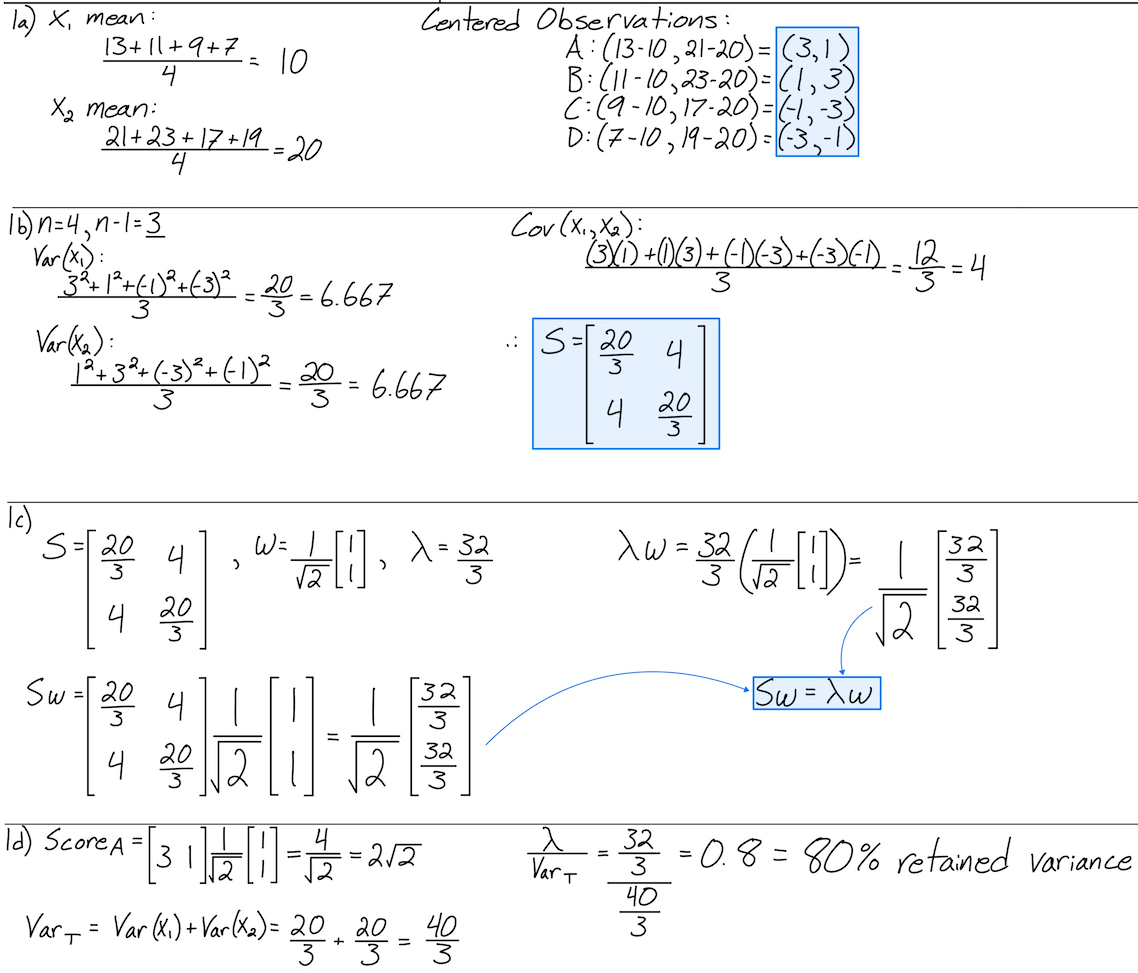
\includegraphics[height=0.27\columnwidth]{HW.png} 
% \end{center}

\begin{center} 
    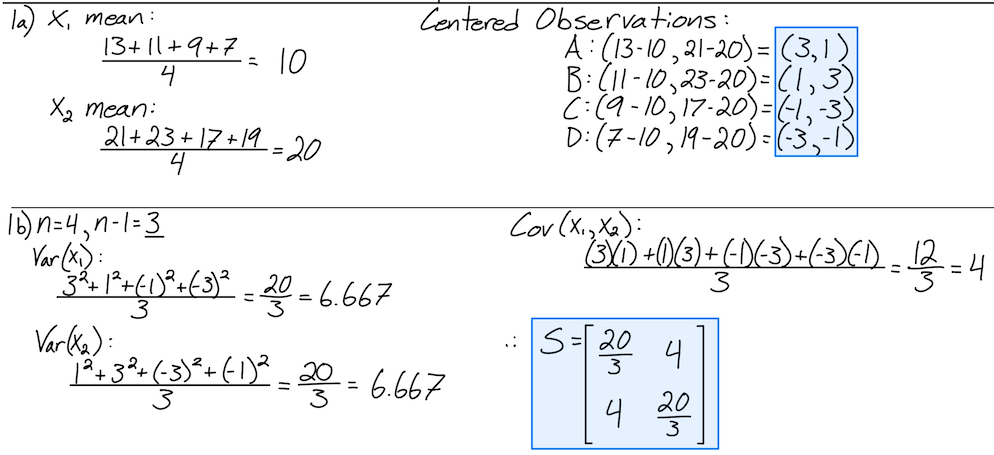
\includegraphics[width=0.49\columnwidth]{HW1.png} 
    \hfill 
    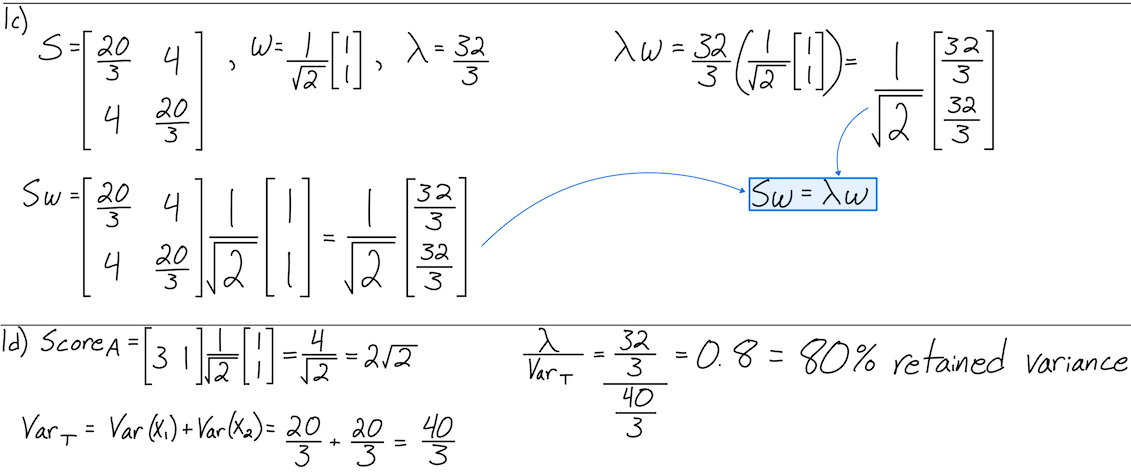
\includegraphics[width=0.49\columnwidth]{HW2.png} 
\end{center}

\columnbreak

\sect{Similarity}
\[
s_{cos}(x,y)=\frac{x^Ty}{\|x\|_2\|y\|_2},\qquad \|x\|_2=\sqrt{\sum_jx_j^2}
\]
Cosine compares direction/proportions and ignores overall magnitude; zero vectors have undefined direction. If a library returns cosine distance, $s=1-d$.
\[
J(A,B)=\frac{|A\cap B|}{|A\cup B|}
\]

% \columnbreak

Jaccard uses binary presence sets: ignores quantities and shared absences; $1$ identical, $0$ no shared presence. No metric is universally best; match metric to the meaning of similarity.

% \columnbreak

\sect{PCA Foundations}
\term{Dimensionality reduction}: represent observations with fewer coordinates. \term{Selection} keeps original features; \term{extraction} creates new features. PCA is linear feature extraction for correlated/redundant measurements.
\[
s^2=\frac{1}{n-1}\sum_i(x_i-\bar x)^2,\qquad \operatorname{Cov}(x,y)=\frac{1}{n-1}\sum_i(x_i-\bar x)(y_i-\bar y)
\]
\[
S=\begin{bmatrix}\operatorname{Var}(x_1)&\operatorname{Cov}(x_1,x_2)\\\operatorname{Cov}(x_1,x_2)&\operatorname{Var}(x_2)\end{bmatrix}
\]
Diagonal $=$ variances; off-diagonal $=$ covariances. Total variance $=\operatorname{tr}(S)=\sum_j\lambda_j$.

\term{Eigen equation:}
\[
Sw=\lambda w,\qquad \|w\|_2=1,\qquad z=w^Tx_c
\]
$w$ = eigenvector/loadings (direction); $\lambda$ = variance captured. PC1 maximizes projected variance; later PCs are orthogonal and maximize remaining variance. Component order: descending $\lambda$. Flipping all signs of a component changes no meaning.
\[
\text{EV fraction}_k=\frac{\lambda_k}{\sum_j\lambda_j},\qquad \text{cumulative retention}_K=\frac{\sum_{k=1}^K\lambda_k}{\sum_j\lambda_j}
\]
Choose $K$ by required retention and cost of losing detail; a 90\% rule is not universal. Standardize first when units/scales differ; HW2B uses sample $s$ (\code{ddof=1}).

\begin{tabular}{@{}p{0.28\linewidth}p{0.66\linewidth}@{}}
\toprule
Term & Meaning \\
\midrule
Loading & Coefficient/direction; \code{pca.components\_}.\\
Score & One record's component coordinates; \code{pca.transform(X)}.\\
Eigenvalue & Variance along a component; \code{explained\_variance\_}.\\
EV ratio & Variance fraction; \code{explained\_variance\_ratio\_}.\\
Reconstruction & Reduced scores $\to$ standardized feature space via \code{inverse\_transform}; undo scaling for original units.\\
\bottomrule
\end{tabular}

\term{Loading interpretation}: compare sign/magnitude within one component. A score's sign indicates alignment with the chosen direction; eigenvector sign is arbitrary. High total retention need not mean every feature/individual reconstructs equally well. New data: use saved training means/scales, then \code{transform}; never refit on the new row.

\sect{Code + Concept Traps}
\begin{itemize}
\item \code{True} behaves as $1$, \code{False} as $0$ in a mean; check missing values first.
\item Permutation shuffles labels/assignments; bootstrap resamples values/units with \code{replace=True}.
\item Seed once before the simulation loop; reseeding inside repeats the same first draw.
\item Independent groups are not paired observations; choose the appropriate permutation type.
\item \code{cdist(..., metric="cosine")} returns distance, not similarity; use $1-d$.
\item Double brackets such as \code{matrix.loc[[anchor]]} preserve a 2D row for \code{cdist}.
\item Remove \code{anchor} before sorting nearest neighbors.
\item Raw numeric, standardized numeric, and binary presence/absence are different representations.
\item \code{fit} learns directions; \code{transform} projects; \code{components\_} are loadings, not scores.
\item Check $\texttt{ddof}=0$ vs $\texttt{ddof}=1$; it changes scales, covariance, and PCA calculations.
\end{itemize}

\sect{Fast Interpretation Starters}
\begin{itemize}
\item \term{Difference}: ``$A-B$ is positive/negative, so $A$ is larger/smaller in [units].''
\item \term{p-value}: ``Under [specific null/simulation], $p$ of simulated statistics were at least this extreme.''
\item \term{CI}: ``The method gives plausible population values from [lower] to [upper], assuming [sampling/resampling assumptions].''
\item \term{Distance}: ``Smaller means closer under this representation and metric; it does not imply universal similarity.''
\item \term{Similarity}: ``Larger means more similar according to [direction / shared presence], not necessarily larger magnitude.''
\item \term{PCA}: ``This loading shows the feature's direction/relative contribution; this score locates one observation in component space.''
\end{itemize}

\sect{Pre-Answer Checklist}
What is one row? What are group/outcome/context? What statistic and subtraction order? What is randomized, and what is fixed? With or without replacement? Raw, standardized, or binary? Distance or similarity? Anchor removed? Which $s$ convention? Does output describe one row, all rows, or a component? What assumptions limit interpretation?

\end{multicols*}
\end{document}
